\documentclass[1p]{elsarticle_modified}
%\bibliographystyle{elsarticle-num}

%\usepackage[colorlinks]{hyperref}
%\usepackage{abbrmath_seonhwa} %\Abb, \Ascr, \Acal ,\Abf, \Afrak
\usepackage{amsfonts}
\usepackage{amssymb}
\usepackage{amsmath}
\usepackage{amsthm}
\usepackage{scalefnt}
\usepackage{amsbsy}
\usepackage{kotex}
\usepackage{caption}
\usepackage{subfig}
\usepackage{color}
\usepackage{graphicx}
\usepackage{xcolor} %% white, black, red, green, blue, cyan, magenta, yellow
\usepackage{float}
\usepackage{setspace}
\usepackage{hyperref}

\usepackage{tikz}
\usetikzlibrary{arrows}

\usepackage{multirow}
\usepackage{array} % fixed length table
\usepackage{hhline}

%%%%%%%%%%%%%%%%%%%%%
\makeatletter
\renewcommand*\env@matrix[1][\arraystretch]{%
	\edef\arraystretch{#1}%
	\hskip -\arraycolsep
	\let\@ifnextchar\new@ifnextchar
	\array{*\c@MaxMatrixCols c}}
\makeatother %https://tex.stackexchange.com/questions/14071/how-can-i-increase-the-line-spacing-in-a-matrix
%%%%%%%%%%%%%%%

\usepackage[normalem]{ulem}

\newcommand{\msout}[1]{\ifmmode\text{\sout{\ensuremath{#1}}}\else\sout{#1}\fi}
%SOURCE: \msout is \stkout macro in https://tex.stackexchange.com/questions/20609/strikeout-in-math-mode

\newcommand{\cancel}[1]{
	\ifmmode
	{\color{red}\msout{#1}}
	\else
	{\color{red}\sout{#1}}
	\fi
}

\newcommand{\add}[1]{
	{\color{blue}\uwave{#1}}
}

\newcommand{\replace}[2]{
	\ifmmode
	{\color{red}\msout{#1}}{\color{blue}\uwave{#2}}
	\else
	{\color{red}\sout{#1}}{\color{blue}\uwave{#2}}
	\fi
}

\newcommand{\Sol}{\mathcal{S}} %segment
\newcommand{\D}{D} %diagram
\newcommand{\A}{\mathcal{A}} %arc


%%%%%%%%%%%%%%%%%%%%%%%%%%%%%5 test

\def\sl{\operatorname{\textup{SL}}(2,\Cbb)}
\def\psl{\operatorname{\textup{PSL}}(2,\Cbb)}
\def\quan{\mkern 1mu \triangleright \mkern 1mu}

\theoremstyle{definition}
\newtheorem{thm}{Theorem}[section]
\newtheorem{prop}[thm]{Proposition}
\newtheorem{lem}[thm]{Lemma}
\newtheorem{ques}[thm]{Question}
\newtheorem{cor}[thm]{Corollary}
\newtheorem{defn}[thm]{Definition}
\newtheorem{exam}[thm]{Example}
\newtheorem{rmk}[thm]{Remark}
\newtheorem{alg}[thm]{Algorithm}

\newcommand{\I}{\sqrt{-1}}
\begin{document}

%\begin{frontmatter}
%
%\title{Boundary parabolic representations of knots up to 8 crossings}
%
%%% Group authors per affiliation:
%\author{Yunhi Cho} 
%\address{Department of Mathematics, University of Seoul, Seoul, Korea}
%\ead{yhcho@uos.ac.kr}
%
%
%\author{Seonhwa Kim} %\fnref{s_kim}}
%\address{Center for Geometry and Physics, Institute for Basic Science, Pohang, 37673, Korea}
%\ead{ryeona17@ibs.re.kr}
%
%\author{Hyuk Kim}
%\address{Department of Mathematical Sciences, Seoul National University, Seoul 08826, Korea}
%\ead{hyukkim@snu.ac.kr}
%
%\author{Seokbeom Yoon}
%\address{Department of Mathematical Sciences, Seoul National University, Seoul, 08826,  Korea}
%\ead{sbyoon15@snu.ac.kr}
%
%\begin{abstract}
%We find all boundary parabolic representation of knots up to 8 crossings.
%
%\end{abstract}
%\begin{keyword}
%    \MSC[2010] 57M25 
%\end{keyword}
%
%\end{frontmatter}

%\linenumbers
%\tableofcontents
%
\newcommand\colored[1]{\textcolor{white}{\rule[-0.35ex]{0.8em}{1.4ex}}\kern-0.8em\color{red} #1}%
%\newcommand\colored[1]{\textcolor{white}{ #1}\kern-2.17ex	\textcolor{white}{ #1}\kern-1.81ex	\textcolor{white}{ #1}\kern-2.15ex\color{red}#1	}

{\Large $\underline{12n_{0661}~(K12n_{0661})}$}

\setlength{\tabcolsep}{10pt}
\renewcommand{\arraystretch}{1.6}
\vspace{1cm}\begin{tabular}{m{100pt}>{\centering\arraybackslash}m{274pt}}
\multirow{5}{120pt}{
	\centering
	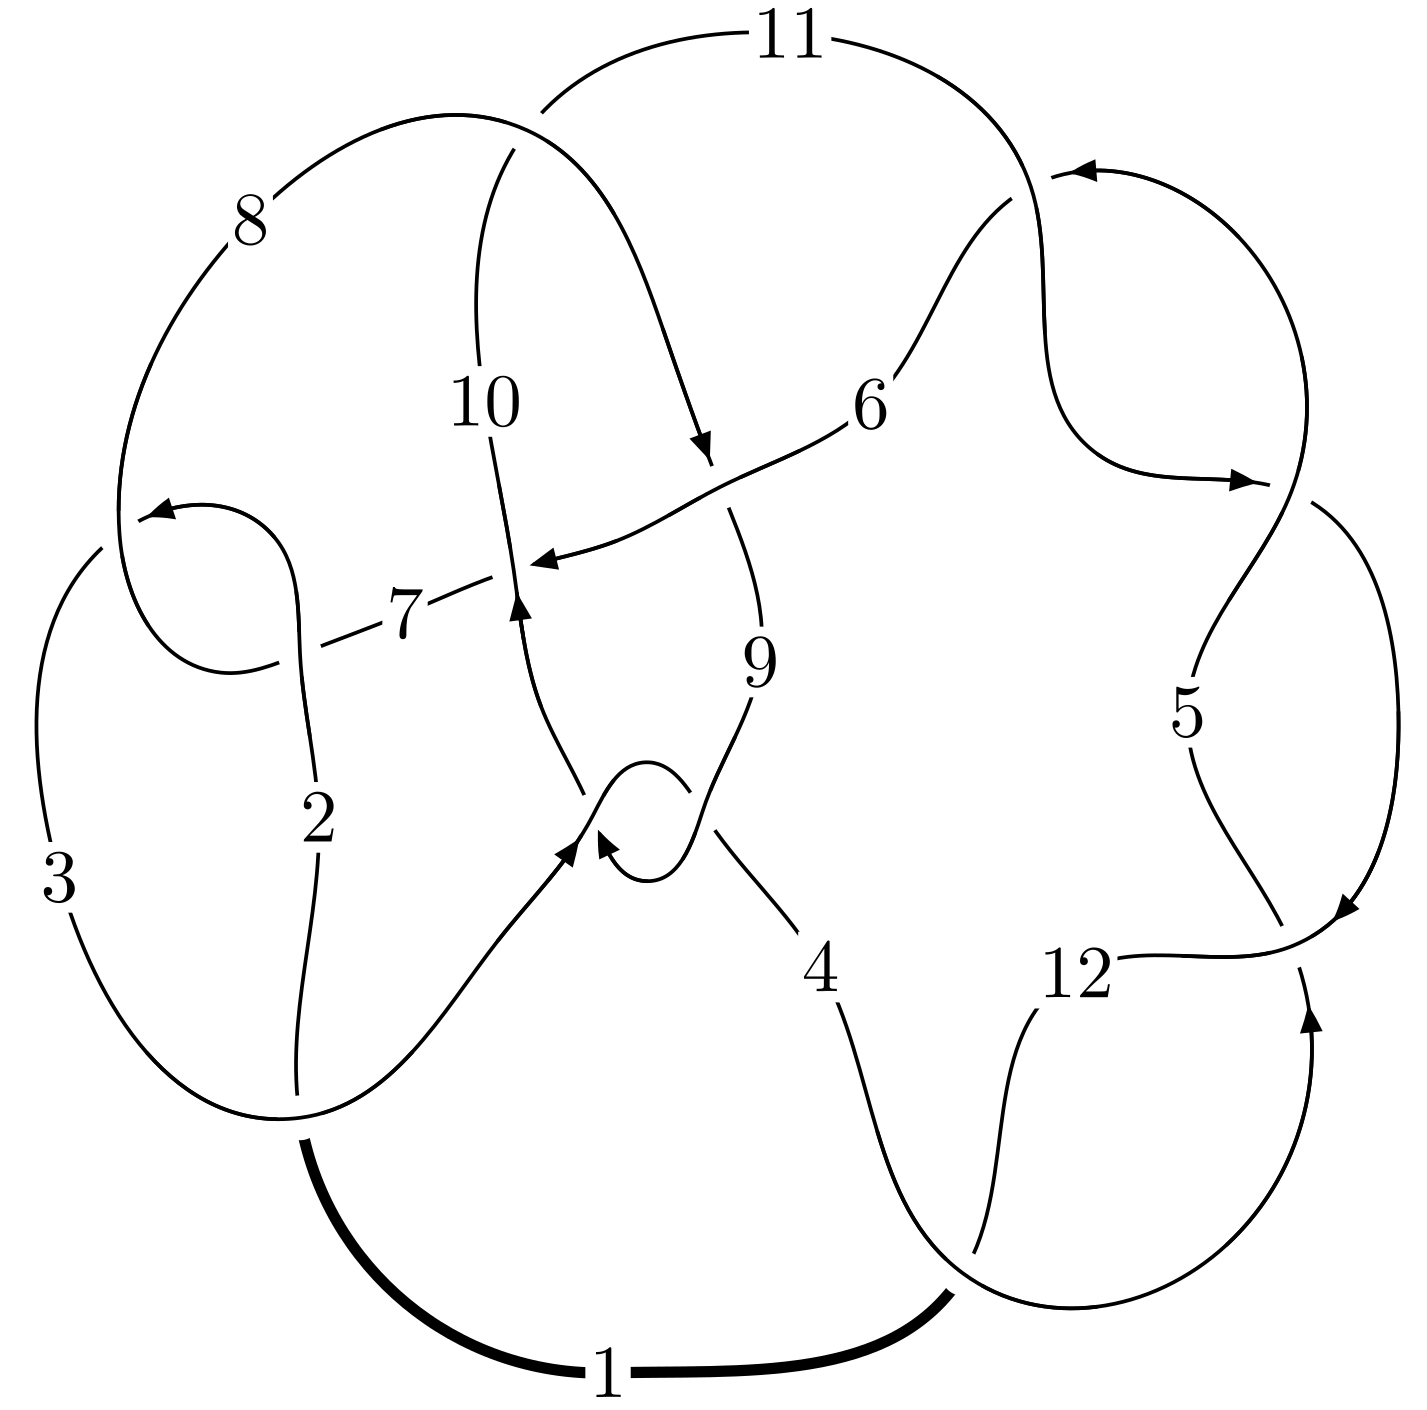
\includegraphics[width=112pt]{../../../GIT/diagram.site/Diagrams/png/2750_12n_0661.png}\\
\ \ \ A knot diagram\footnotemark}&
\allowdisplaybreaks
\textbf{Linearized knot diagam} \\
\cline{2-2}
 &
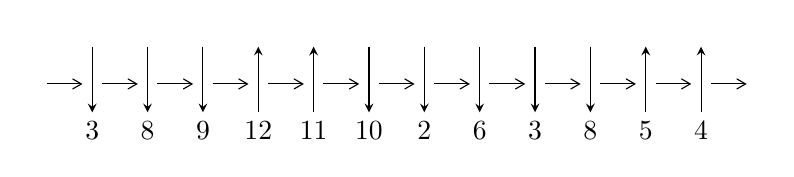
\begin{tikzpicture}[x=20pt, y=17pt]
	% nodes
	\node (C0) at (0, 0) {};
	\node (C1) at (1, 0) {};
	\node (C1U) at (1, +1) {};
	\node (C1D) at (1, -1) {3};

	\node (C2) at (2, 0) {};
	\node (C2U) at (2, +1) {};
	\node (C2D) at (2, -1) {8};

	\node (C3) at (3, 0) {};
	\node (C3U) at (3, +1) {};
	\node (C3D) at (3, -1) {9};

	\node (C4) at (4, 0) {};
	\node (C4U) at (4, +1) {};
	\node (C4D) at (4, -1) {12};

	\node (C5) at (5, 0) {};
	\node (C5U) at (5, +1) {};
	\node (C5D) at (5, -1) {11};

	\node (C6) at (6, 0) {};
	\node (C6U) at (6, +1) {};
	\node (C6D) at (6, -1) {10};

	\node (C7) at (7, 0) {};
	\node (C7U) at (7, +1) {};
	\node (C7D) at (7, -1) {2};

	\node (C8) at (8, 0) {};
	\node (C8U) at (8, +1) {};
	\node (C8D) at (8, -1) {6};

	\node (C9) at (9, 0) {};
	\node (C9U) at (9, +1) {};
	\node (C9D) at (9, -1) {3};

	\node (C10) at (10, 0) {};
	\node (C10U) at (10, +1) {};
	\node (C10D) at (10, -1) {8};

	\node (C11) at (11, 0) {};
	\node (C11U) at (11, +1) {};
	\node (C11D) at (11, -1) {5};

	\node (C12) at (12, 0) {};
	\node (C12U) at (12, +1) {};
	\node (C12D) at (12, -1) {4};
	\node (C13) at (13, 0) {};

	% arrows
	\draw[->,>={angle 60}]
	(C0) edge (C1) (C1) edge (C2) (C2) edge (C3) (C3) edge (C4) (C4) edge (C5) (C5) edge (C6) (C6) edge (C7) (C7) edge (C8) (C8) edge (C9) (C9) edge (C10) (C10) edge (C11) (C11) edge (C12) (C12) edge (C13) ;	\draw[->,>=stealth]
	(C1U) edge (C1D) (C2U) edge (C2D) (C3U) edge (C3D) (C4D) edge (C4U) (C5D) edge (C5U) (C6U) edge (C6D) (C7U) edge (C7D) (C8U) edge (C8D) (C9U) edge (C9D) (C10U) edge (C10D) (C11D) edge (C11U) (C12D) edge (C12U) ;
	\end{tikzpicture} \\
\hhline{~~} \\& 
\textbf{Solving Sequence} \\ \cline{2-2} 
 &
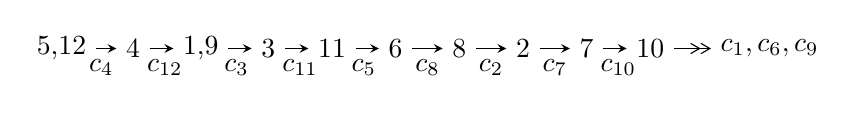
\begin{tikzpicture}[x=23pt, y=7pt]
	% node
	\node (A0) at (-1/8, 0) {5,12};
	\node (A1) at (1, 0) {4};
	\node (A2) at (33/16, 0) {1,9};
	\node (A3) at (25/8, 0) {3};
	\node (A4) at (33/8, 0) {11};
	\node (A5) at (41/8, 0) {6};
	\node (A6) at (49/8, 0) {8};
	\node (A7) at (57/8, 0) {2};
	\node (A8) at (65/8, 0) {7};
	\node (A9) at (73/8, 0) {10};
	\node (C1) at (1/2, -1) {$c_{4}$};
	\node (C2) at (3/2, -1) {$c_{12}$};
	\node (C3) at (21/8, -1) {$c_{3}$};
	\node (C4) at (29/8, -1) {$c_{11}$};
	\node (C5) at (37/8, -1) {$c_{5}$};
	\node (C6) at (45/8, -1) {$c_{8}$};
	\node (C7) at (53/8, -1) {$c_{2}$};
	\node (C8) at (61/8, -1) {$c_{7}$};
	\node (C9) at (69/8, -1) {$c_{10}$};
	\node (A10) at (11, 0) {$c_{1},c_{6},c_{9}$};

	% edge
	\draw[->,>=stealth]	
	(A0) edge (A1) (A1) edge (A2) (A2) edge (A3) (A3) edge (A4) (A4) edge (A5) (A5) edge (A6) (A6) edge (A7) (A7) edge (A8) (A8) edge (A9) ;
	\draw[->>,>={angle 60}]	
	(A9) edge (A10);
\end{tikzpicture} \\ 

\end{tabular} \\

\footnotetext{
The image of knot diagram is generated by the software ``\textbf{Draw programme}" developed by Andrew Bartholomew(\url{http://www.layer8.co.uk/maths/draw/index.htm\#Running-draw}), where we modified some parts for our purpose(\url{https://github.com/CATsTAILs/LinksPainter}).
}\phantom \\ \newline 
\centering \textbf{Ideals for irreducible components\footnotemark of $X_{\text{par}}$} 
 
\begin{align*}
I^u_{1}&=\langle 
-1.88753\times10^{16} u^{26}-7.56446\times10^{16} u^{25}+\cdots+3.81765\times10^{17} b-2.36711\times10^{17},\\
\phantom{I^u_{1}}&\phantom{= \langle  }7.72254\times10^{17} u^{26}+1.53152\times10^{18} u^{25}+\cdots+3.81765\times10^{17} a+1.17596\times10^{19},\;u^{27}+2 u^{26}+\cdots+13 u+1\rangle \\
I^u_{2}&=\langle 
- u^{12}+u^{11}-8 u^{10}+7 u^9-24 u^8+17 u^7-33 u^6+15 u^5-19 u^4-2 u^2+b-4 u,\\
\phantom{I^u_{2}}&\phantom{= \langle  }u^{12}- u^{11}+8 u^{10}-7 u^9+24 u^8-17 u^7+33 u^6-15 u^5+20 u^4- u^3+5 u^2+a+2 u+2,\\
\phantom{I^u_{2}}&\phantom{= \langle  }u^{13}- u^{12}+9 u^{11}-8 u^{10}+31 u^9-23 u^8+50 u^7-26 u^6+36 u^5-5 u^4+8 u^3+6 u^2+1\rangle \\
\\
\end{align*}
\raggedright * 2 irreducible components of $\dim_{\mathbb{C}}=0$, with total 40 representations.\\
\footnotetext{All coefficients of polynomials are rational numbers. But the coefficients are sometimes approximated in decimal forms when there is not enough margin.}
\newpage
\renewcommand{\arraystretch}{1}
\centering \section*{I. $I^u_{1}= \langle -1.89\times10^{16} u^{26}-7.56\times10^{16} u^{25}+\cdots+3.82\times10^{17} b-2.37\times10^{17},\;7.72\times10^{17} u^{26}+1.53\times10^{18} u^{25}+\cdots+3.82\times10^{17} a+1.18\times10^{19},\;u^{27}+2 u^{26}+\cdots+13 u+1 \rangle$}
\flushleft \textbf{(i) Arc colorings}\\
\begin{tabular}{m{7pt} m{180pt} m{7pt} m{180pt} }
\flushright $a_{5}=$&$\begin{pmatrix}1\\0\end{pmatrix}$ \\
\flushright $a_{12}=$&$\begin{pmatrix}0\\u\end{pmatrix}$ \\
\flushright $a_{4}=$&$\begin{pmatrix}1\\u^2\end{pmatrix}$ \\
\flushright $a_{1}=$&$\begin{pmatrix}u\\u^3+u\end{pmatrix}$ \\
\flushright $a_{9}=$&$\begin{pmatrix}-2.02285 u^{26}-4.01168 u^{25}+\cdots+52.8694 u-30.8031\\0.0494422 u^{26}+0.198144 u^{25}+\cdots-4.98870 u+0.620042\end{pmatrix}$ \\
\flushright $a_{3}=$&$\begin{pmatrix}2.30870 u^{26}+4.40950 u^{25}+\cdots-64.8476 u+32.0288\\-0.147916 u^{26}-0.156483 u^{25}+\cdots+5.40884 u-0.571583\end{pmatrix}$ \\
\flushright $a_{11}=$&$\begin{pmatrix}- u\\u\end{pmatrix}$ \\
\flushright $a_{6}=$&$\begin{pmatrix}u^2+1\\- u^2\end{pmatrix}$ \\
\flushright $a_{8}=$&$\begin{pmatrix}-1.84488 u^{26}-3.63901 u^{25}+\cdots+46.6032 u-30.4259\\-0.0335197 u^{26}+0.124979 u^{25}+\cdots-3.47040 u+0.729526\end{pmatrix}$ \\
\flushright $a_{2}=$&$\begin{pmatrix}5.51519 u^{26}+10.4146 u^{25}+\cdots-140.640 u+79.5005\\-0.539565 u^{26}-0.738431 u^{25}+\cdots+12.0070 u-1.51404\end{pmatrix}$ \\
\flushright $a_{7}=$&$\begin{pmatrix}6.44254 u^{26}+12.6459 u^{25}+\cdots-163.824 u+94.6771\\0.187806 u^{26}+0.130509 u^{25}+\cdots+3.17687 u-2.60252\end{pmatrix}$ \\
\flushright $a_{10}=$&$\begin{pmatrix}-4.41532 u^{26}-8.66985 u^{25}+\cdots+116.266 u-63.9888\\-0.0901988 u^{26}-0.0255952 u^{25}+\cdots+1.47740 u+1.99746\end{pmatrix}$\\&\end{tabular}
\flushleft \textbf{(ii) Obstruction class $= -1$}\\~\\
\flushleft \textbf{(iii) Cusp Shapes $= -\frac{512696248127693729}{381765450474394411} u^{26}-\frac{1173688396623260553}{381765450474394411} u^{25}+\cdots+\frac{23974986416882589793}{381765450474394411} u-\frac{7032162693009829437}{381765450474394411}$}\\~\\
\newpage\renewcommand{\arraystretch}{1}
\flushleft \textbf{(iv) u-Polynomials at the component}\newline \\
\begin{tabular}{m{50pt}|m{274pt}}
Crossings & \hspace{64pt}u-Polynomials at each crossing \\
\hline $$\begin{aligned}c_{1}\end{aligned}$$&$\begin{aligned}
&u^{27}+43 u^{26}+\cdots+32307 u+14641
\end{aligned}$\\
\hline $$\begin{aligned}c_{2},c_{7}\end{aligned}$$&$\begin{aligned}
&u^{27}+u^{26}+\cdots-451 u-121
\end{aligned}$\\
\hline $$\begin{aligned}c_{3},c_{9}\end{aligned}$$&$\begin{aligned}
&u^{27}- u^{26}+\cdots+57 u+173
\end{aligned}$\\
\hline $$\begin{aligned}c_{4},c_{5},c_{11}\\c_{12}\end{aligned}$$&$\begin{aligned}
&u^{27}+2 u^{26}+\cdots+13 u+1
\end{aligned}$\\
\hline $$\begin{aligned}c_{6}\end{aligned}$$&$\begin{aligned}
&u^{27}-30 u^{25}+\cdots+20449 u-8017
\end{aligned}$\\
\hline $$\begin{aligned}c_{8}\end{aligned}$$&$\begin{aligned}
&u^{27}-5 u^{26}+\cdots-38 u+7
\end{aligned}$\\
\hline $$\begin{aligned}c_{10}\end{aligned}$$&$\begin{aligned}
&u^{27}-22 u^{25}+\cdots+125 u-21
\end{aligned}$\\
\hline
\end{tabular}\\~\\
\newpage\renewcommand{\arraystretch}{1}
\flushleft \textbf{(v) Riley Polynomials at the component}\newline \\
\begin{tabular}{m{50pt}|m{274pt}}
Crossings & \hspace{64pt}Riley Polynomials at each crossing \\
\hline $$\begin{aligned}c_{1}\end{aligned}$$&$\begin{aligned}
&y^{27}-111 y^{26}+\cdots+6730511623 y-214358881
\end{aligned}$\\
\hline $$\begin{aligned}c_{2},c_{7}\end{aligned}$$&$\begin{aligned}
&y^{27}-43 y^{26}+\cdots+32307 y-14641
\end{aligned}$\\
\hline $$\begin{aligned}c_{3},c_{9}\end{aligned}$$&$\begin{aligned}
&y^{27}-11 y^{26}+\cdots+147185 y-29929
\end{aligned}$\\
\hline $$\begin{aligned}c_{4},c_{5},c_{11}\\c_{12}\end{aligned}$$&$\begin{aligned}
&y^{27}+38 y^{26}+\cdots+237 y-1
\end{aligned}$\\
\hline $$\begin{aligned}c_{6}\end{aligned}$$&$\begin{aligned}
&y^{27}-60 y^{26}+\cdots-129367431 y-64272289
\end{aligned}$\\
\hline $$\begin{aligned}c_{8}\end{aligned}$$&$\begin{aligned}
&y^{27}-7 y^{26}+\cdots+1402 y-49
\end{aligned}$\\
\hline $$\begin{aligned}c_{10}\end{aligned}$$&$\begin{aligned}
&y^{27}-44 y^{26}+\cdots-965 y-441
\end{aligned}$\\
\hline
\end{tabular}\\~\\
\newpage\flushleft \textbf{(vi) Complex Volumes and Cusp Shapes}
$$\begin{array}{c|c|c}  
\text{Solutions to }I^u_{1}& \I (\text{vol} + \sqrt{-1}CS) & \text{Cusp shape}\\
 \hline 
\begin{aligned}
u &= \phantom{-}0.038928 + 1.096540 I \\
a &= \phantom{-}0.339795 - 0.956003 I \\
b &= -0.047794 + 0.583517 I\end{aligned}
 & -1.18227 + 2.78711 I & -8.53482 - 4.99224 I \\ \hline\begin{aligned}
u &= \phantom{-}0.038928 - 1.096540 I \\
a &= \phantom{-}0.339795 + 0.956003 I \\
b &= -0.047794 - 0.583517 I\end{aligned}
 & -1.18227 - 2.78711 I & -8.53482 + 4.99224 I \\ \hline\begin{aligned}
u &= -0.060221 + 1.114710 I \\
a &= -0.818699 + 1.150860 I \\
b &= \phantom{-}0.00282 - 2.15523 I\end{aligned}
 & -11.46510 - 0.44076 I & -9.43738 - 0.19503 I \\ \hline\begin{aligned}
u &= -0.060221 - 1.114710 I \\
a &= -0.818699 - 1.150860 I \\
b &= \phantom{-}0.00282 + 2.15523 I\end{aligned}
 & -11.46510 + 0.44076 I & -9.43738 + 0.19503 I \\ \hline\begin{aligned}
u &= -1.18869\phantom{ +0.000000I} \\
a &= -0.494164\phantom{ +0.000000I} \\
b &= \phantom{-}0.786510\phantom{ +0.000000I}\end{aligned}
 & -9.76195\phantom{ +0.000000I} & -9.69870\phantom{ +0.000000I} \\ \hline\begin{aligned}
u &= -0.319861 + 0.734406 I \\
a &= \phantom{-}1.137130 - 0.483412 I \\
b &= \phantom{-}0.082638 - 0.422987 I\end{aligned}
 & -2.86657 - 2.08543 I & -10.74476 + 3.06559 I \\ \hline\begin{aligned}
u &= -0.319861 - 0.734406 I \\
a &= \phantom{-}1.137130 + 0.483412 I \\
b &= \phantom{-}0.082638 + 0.422987 I\end{aligned}
 & -2.86657 + 2.08543 I & -10.74476 - 3.06559 I \\ \hline\begin{aligned}
u &= \phantom{-}0.374600 + 0.697774 I \\
a &= -0.765943 - 0.335826 I \\
b &= \phantom{-}0.067516 + 0.335617 I\end{aligned}
 & -0.19323 + 1.53182 I & -2.51900 - 3.03384 I \\ \hline\begin{aligned}
u &= \phantom{-}0.374600 - 0.697774 I \\
a &= -0.765943 + 0.335826 I \\
b &= \phantom{-}0.067516 - 0.335617 I\end{aligned}
 & -0.19323 - 1.53182 I & -2.51900 + 3.03384 I \\ \hline\begin{aligned}
u &= \phantom{-}0.445707 + 1.146890 I \\
a &= -0.198922 + 0.327688 I \\
b &= \phantom{-}0.275375 + 0.416461 I\end{aligned}
 & -0.824285 + 1.070290 I & -8.64760 + 1.85610 I\\
 \hline 
 \end{array}$$\newpage$$\begin{array}{c|c|c}  
\text{Solutions to }I^u_{1}& \I (\text{vol} + \sqrt{-1}CS) & \text{Cusp shape}\\
 \hline 
\begin{aligned}
u &= \phantom{-}0.445707 - 1.146890 I \\
a &= -0.198922 - 0.327688 I \\
b &= \phantom{-}0.275375 - 0.416461 I\end{aligned}
 & -0.824285 - 1.070290 I & -8.64760 - 1.85610 I \\ \hline\begin{aligned}
u &= -0.803778 + 1.109510 I \\
a &= -0.585598 + 0.655588 I \\
b &= -0.0328420 - 0.1176830 I\end{aligned}
 & -13.1170 - 6.5745 I & -9.22636 + 4.44172 I \\ \hline\begin{aligned}
u &= -0.803778 - 1.109510 I \\
a &= -0.585598 - 0.655588 I \\
b &= -0.0328420 + 0.1176830 I\end{aligned}
 & -13.1170 + 6.5745 I & -9.22636 - 4.44172 I \\ \hline\begin{aligned}
u &= -0.11687 + 1.62312 I \\
a &= -1.64946 + 0.43051 I \\
b &= \phantom{-}3.21083 - 0.53420 I\end{aligned}
 & -11.01260 - 3.84052 I & -10.07314 + 2.86056 I \\ \hline\begin{aligned}
u &= -0.11687 - 1.62312 I \\
a &= -1.64946 - 0.43051 I \\
b &= \phantom{-}3.21083 + 0.53420 I\end{aligned}
 & -11.01260 + 3.84052 I & -10.07314 - 2.86056 I \\ \hline\begin{aligned}
u &= \phantom{-}0.11486 + 1.65386 I \\
a &= \phantom{-}1.306150 - 0.183873 I \\
b &= -2.63732 + 0.04241 I\end{aligned}
 & -8.53404 + 3.33702 I & -6.52566 + 0. I\phantom{ +0.000000I} \\ \hline\begin{aligned}
u &= \phantom{-}0.11486 - 1.65386 I \\
a &= \phantom{-}1.306150 + 0.183873 I \\
b &= -2.63732 - 0.04241 I\end{aligned}
 & -8.53404 - 3.33702 I & -6.52566 + 0. I\phantom{ +0.000000I} \\ \hline\begin{aligned}
u &= \phantom{-}0.314955 + 0.040141 I \\
a &= -1.52461 - 0.75675 I \\
b &= -0.092808 + 1.092340 I\end{aligned}
 & \phantom{-}2.49846 + 1.59988 I & \phantom{-}3.26170 - 4.46285 I \\ \hline\begin{aligned}
u &= \phantom{-}0.314955 - 0.040141 I \\
a &= -1.52461 + 0.75675 I \\
b &= -0.092808 - 1.092340 I\end{aligned}
 & \phantom{-}2.49846 - 1.59988 I & \phantom{-}3.26170 + 4.46285 I \\ \hline\begin{aligned}
u &= -0.291278\phantom{ +0.000000I} \\
a &= -0.909250\phantom{ +0.000000I} \\
b &= -0.503041\phantom{ +0.000000I}\end{aligned}
 & -0.940177\phantom{ +0.000000I} & -10.5360\phantom{ +0.000000I}\\
 \hline 
 \end{array}$$\newpage$$\begin{array}{c|c|c}  
\text{Solutions to }I^u_{1}& \I (\text{vol} + \sqrt{-1}CS) & \text{Cusp shape}\\
 \hline 
\begin{aligned}
u &= -0.02099 + 1.78831 I \\
a &= \phantom{-}1.199340 + 0.558142 I \\
b &= -2.31418 - 0.09316 I\end{aligned}
 & \phantom{-}17.2683 - 0.8391 I & \phantom{-0.000000 } 0 \\ \hline\begin{aligned}
u &= -0.02099 - 1.78831 I \\
a &= \phantom{-}1.199340 - 0.558142 I \\
b &= -2.31418 + 0.09316 I\end{aligned}
 & \phantom{-}17.2683 + 0.8391 I & \phantom{-0.000000 } 0 \\ \hline\begin{aligned}
u &= -0.23930 + 1.77241 I \\
a &= \phantom{-}1.50180 + 0.12267 I \\
b &= -2.92542 - 0.18853 I\end{aligned}
 & \phantom{-}16.5332 - 10.9055 I & \phantom{-0.000000 } 0 \\ \hline\begin{aligned}
u &= -0.23930 - 1.77241 I \\
a &= \phantom{-}1.50180 - 0.12267 I \\
b &= -2.92542 + 0.18853 I\end{aligned}
 & \phantom{-}16.5332 + 10.9055 I & \phantom{-0.000000 } 0 \\ \hline\begin{aligned}
u &= \phantom{-}0.04590 + 1.81690 I \\
a &= -1.197200 - 0.034284 I \\
b &= \phantom{-}2.33171 - 0.21126 I\end{aligned}
 & -12.44700 + 3.08894 I & \phantom{-0.000000 } 0 \\ \hline\begin{aligned}
u &= \phantom{-}0.04590 - 1.81690 I \\
a &= -1.197200 + 0.034284 I \\
b &= \phantom{-}2.33171 + 0.21126 I\end{aligned}
 & -12.44700 - 3.08894 I & \phantom{-0.000000 } 0 \\ \hline\begin{aligned}
u &= -0.0678774\phantom{ +0.000000I} \\
a &= -33.0841\phantom{ +0.000000I} \\
b &= \phantom{-}0.875475\phantom{ +0.000000I}\end{aligned}
 & -7.70070\phantom{ +0.000000I} & -21.8510\phantom{ +0.000000I}\\
 \hline 
 \end{array}$$\newpage\newpage\renewcommand{\arraystretch}{1}
\centering \section*{II. $I^u_{2}= \langle - u^{12}+u^{11}+\cdots+b-4 u,\;u^{12}- u^{11}+\cdots+a+2,\;u^{13}- u^{12}+\cdots+6 u^2+1 \rangle$}
\flushleft \textbf{(i) Arc colorings}\\
\begin{tabular}{m{7pt} m{180pt} m{7pt} m{180pt} }
\flushright $a_{5}=$&$\begin{pmatrix}1\\0\end{pmatrix}$ \\
\flushright $a_{12}=$&$\begin{pmatrix}0\\u\end{pmatrix}$ \\
\flushright $a_{4}=$&$\begin{pmatrix}1\\u^2\end{pmatrix}$ \\
\flushright $a_{1}=$&$\begin{pmatrix}u\\u^3+u\end{pmatrix}$ \\
\flushright $a_{9}=$&$\begin{pmatrix}- u^{12}+u^{11}+\cdots-2 u-2\\u^{12}- u^{11}+8 u^{10}-7 u^9+24 u^8-17 u^7+33 u^6-15 u^5+19 u^4+2 u^2+4 u\end{pmatrix}$ \\
\flushright $a_{3}=$&$\begin{pmatrix}u^{12}- u^{11}+\cdots+9 u^2+4 u\\u^9- u^8+6 u^7-5 u^6+12 u^5-7 u^4+9 u^3+u+2\end{pmatrix}$ \\
\flushright $a_{11}=$&$\begin{pmatrix}- u\\u\end{pmatrix}$ \\
\flushright $a_{6}=$&$\begin{pmatrix}u^2+1\\- u^2\end{pmatrix}$ \\
\flushright $a_{8}=$&$\begin{pmatrix}- u^{12}+u^{11}+\cdots+u-2\\2 u^{12}-2 u^{11}+\cdots+2 u^2+5 u\end{pmatrix}$ \\
\flushright $a_{2}=$&$\begin{pmatrix}2 u^{12}-3 u^{11}+\cdots+u-1\\u^{11}+7 u^9+17 u^7+u^6+17 u^5+4 u^4+10 u^3+5 u^2+5 u+2\end{pmatrix}$ \\
\flushright $a_{7}=$&$\begin{pmatrix}u^{12}- u^{11}+\cdots-6 u+3\\- u^{12}-6 u^{10}+\cdots-2 u-1\end{pmatrix}$ \\
\flushright $a_{10}=$&$\begin{pmatrix}- u^{10}+2 u^9-8 u^8+13 u^7-24 u^6+29 u^5-31 u^4+23 u^3-13 u^2+3 u\\- u^{12}+2 u^{11}+\cdots-3 u+1\end{pmatrix}$\\&\end{tabular}
\flushleft \textbf{(ii) Obstruction class $= 1$}\\~\\
\flushleft \textbf{(iii) Cusp Shapes $= 2 u^{12}-4 u^{11}+19 u^{10}-31 u^9+70 u^8-87 u^7+119 u^6-101 u^5+82 u^4-37 u^3+7 u^2+u-11$}\\~\\
\newpage\renewcommand{\arraystretch}{1}
\flushleft \textbf{(iv) u-Polynomials at the component}\newline \\
\begin{tabular}{m{50pt}|m{274pt}}
Crossings & \hspace{64pt}u-Polynomials at each crossing \\
\hline $$\begin{aligned}c_{1}\end{aligned}$$&$\begin{aligned}
&u^{13}-12 u^{12}+\cdots+6 u-1
\end{aligned}$\\
\hline $$\begin{aligned}c_{2}\end{aligned}$$&$\begin{aligned}
&u^{13}-6 u^{11}+\cdots+3 u^2-1
\end{aligned}$\\
\hline $$\begin{aligned}c_{3}\end{aligned}$$&$\begin{aligned}
&u^{13}+4 u^{11}+u^{10}+3 u^9+3 u^8-3 u^7+u^6- u^5-5 u^4+2 u^3-4 u^2-1
\end{aligned}$\\
\hline $$\begin{aligned}c_{4},c_{5}\end{aligned}$$&$\begin{aligned}
&u^{13}- u^{12}+\cdots+6 u^2+1
\end{aligned}$\\
\hline $$\begin{aligned}c_{6}\end{aligned}$$&$\begin{aligned}
&u^{13}- u^{12}+\cdots-4 u+1
\end{aligned}$\\
\hline $$\begin{aligned}c_{7}\end{aligned}$$&$\begin{aligned}
&u^{13}-6 u^{11}+\cdots-3 u^2+1
\end{aligned}$\\
\hline $$\begin{aligned}c_{8}\end{aligned}$$&$\begin{aligned}
&u^{13}+4 u^{12}+\cdots- u-1
\end{aligned}$\\
\hline $$\begin{aligned}c_{9}\end{aligned}$$&$\begin{aligned}
&u^{13}+4 u^{11}- u^{10}+3 u^9-3 u^8-3 u^7- u^6- u^5+5 u^4+2 u^3+4 u^2+1
\end{aligned}$\\
\hline $$\begin{aligned}c_{10}\end{aligned}$$&$\begin{aligned}
&u^{13}+5 u^{12}+\cdots+4 u+1
\end{aligned}$\\
\hline $$\begin{aligned}c_{11},c_{12}\end{aligned}$$&$\begin{aligned}
&u^{13}+u^{12}+\cdots-6 u^2-1
\end{aligned}$\\
\hline
\end{tabular}\\~\\
\newpage\renewcommand{\arraystretch}{1}
\flushleft \textbf{(v) Riley Polynomials at the component}\newline \\
\begin{tabular}{m{50pt}|m{274pt}}
Crossings & \hspace{64pt}Riley Polynomials at each crossing \\
\hline $$\begin{aligned}c_{1}\end{aligned}$$&$\begin{aligned}
&y^{13}-16 y^{12}+\cdots-10 y-1
\end{aligned}$\\
\hline $$\begin{aligned}c_{2},c_{7}\end{aligned}$$&$\begin{aligned}
&y^{13}-12 y^{12}+\cdots+6 y-1
\end{aligned}$\\
\hline $$\begin{aligned}c_{3},c_{9}\end{aligned}$$&$\begin{aligned}
&y^{13}+8 y^{12}+\cdots-8 y-1
\end{aligned}$\\
\hline $$\begin{aligned}c_{4},c_{5},c_{11}\\c_{12}\end{aligned}$$&$\begin{aligned}
&y^{13}+17 y^{12}+\cdots-12 y-1
\end{aligned}$\\
\hline $$\begin{aligned}c_{6}\end{aligned}$$&$\begin{aligned}
&y^{13}-5 y^{12}+\cdots-4 y-1
\end{aligned}$\\
\hline $$\begin{aligned}c_{8}\end{aligned}$$&$\begin{aligned}
&y^{13}+4 y^{12}+\cdots+5 y-1
\end{aligned}$\\
\hline $$\begin{aligned}c_{10}\end{aligned}$$&$\begin{aligned}
&y^{13}-17 y^{12}+\cdots-10 y-1
\end{aligned}$\\
\hline
\end{tabular}\\~\\
\newpage\flushleft \textbf{(vi) Complex Volumes and Cusp Shapes}
$$\begin{array}{c|c|c}  
\text{Solutions to }I^u_{2}& \I (\text{vol} + \sqrt{-1}CS) & \text{Cusp shape}\\
 \hline 
\begin{aligned}
u &= \phantom{-}0.133548 + 1.037260 I \\
a &= -0.533043 + 0.773593 I \\
b &= \phantom{-}0.502915 - 0.004440 I\end{aligned}
 & -0.15268 + 2.04240 I & -3.65004 - 2.96160 I \\ \hline\begin{aligned}
u &= \phantom{-}0.133548 - 1.037260 I \\
a &= -0.533043 - 0.773593 I \\
b &= \phantom{-}0.502915 + 0.004440 I\end{aligned}
 & -0.15268 - 2.04240 I & -3.65004 + 2.96160 I \\ \hline\begin{aligned}
u &= \phantom{-}0.595022 + 0.705190 I \\
a &= -0.707954 - 0.450630 I \\
b &= \phantom{-}0.334443 - 0.017859 I\end{aligned}
 & -0.95065 + 2.25169 I & -8.21474 - 6.15376 I \\ \hline\begin{aligned}
u &= \phantom{-}0.595022 - 0.705190 I \\
a &= -0.707954 + 0.450630 I \\
b &= \phantom{-}0.334443 + 0.017859 I\end{aligned}
 & -0.95065 - 2.25169 I & -8.21474 + 6.15376 I \\ \hline\begin{aligned}
u &= -0.18499 + 1.50758 I \\
a &= -1.06900 + 1.10979 I \\
b &= \phantom{-}1.96964 - 2.19015 I\end{aligned}
 & -12.75340 - 2.45911 I & -12.84063 + 2.25061 I \\ \hline\begin{aligned}
u &= -0.18499 - 1.50758 I \\
a &= -1.06900 - 1.10979 I \\
b &= \phantom{-}1.96964 + 2.19015 I\end{aligned}
 & -12.75340 + 2.45911 I & -12.84063 - 2.25061 I \\ \hline\begin{aligned}
u &= -0.458933\phantom{ +0.000000I} \\
a &= -3.86284\phantom{ +0.000000I} \\
b &= \phantom{-}0.172095\phantom{ +0.000000I}\end{aligned}
 & -7.33687\phantom{ +0.000000I} & \phantom{-}0.945020\phantom{ +0.000000I} \\ \hline\begin{aligned}
u &= \phantom{-}0.01093 + 1.55303 I \\
a &= \phantom{-}0.566263 - 0.677012 I \\
b &= -1.203680 + 0.099823 I\end{aligned}
 & -4.99307 - 1.29173 I & -8.47906 + 1.03783 I \\ \hline\begin{aligned}
u &= \phantom{-}0.01093 - 1.55303 I \\
a &= \phantom{-}0.566263 + 0.677012 I \\
b &= -1.203680 - 0.099823 I\end{aligned}
 & -4.99307 + 1.29173 I & -8.47906 - 1.03783 I \\ \hline\begin{aligned}
u &= \phantom{-}0.047246 + 0.397006 I \\
a &= -1.63460 - 0.77504 I \\
b &= \phantom{-}0.15026 + 1.40825 I\end{aligned}
 & \phantom{-}1.86356 - 1.48404 I & -10.17394 + 1.43832 I\\
 \hline 
 \end{array}$$\newpage$$\begin{array}{c|c|c}  
\text{Solutions to }I^u_{2}& \I (\text{vol} + \sqrt{-1}CS) & \text{Cusp shape}\\
 \hline 
\begin{aligned}
u &= \phantom{-}0.047246 - 0.397006 I \\
a &= -1.63460 + 0.77504 I \\
b &= \phantom{-}0.15026 - 1.40825 I\end{aligned}
 & \phantom{-}1.86356 + 1.48404 I & -10.17394 - 1.43832 I \\ \hline\begin{aligned}
u &= \phantom{-}0.12770 + 1.61697 I \\
a &= \phantom{-}1.309750 - 0.068445 I \\
b &= -2.83963 + 0.06093 I\end{aligned}
 & -8.95416 + 4.67635 I & -7.61410 - 5.21153 I \\ \hline\begin{aligned}
u &= \phantom{-}0.12770 - 1.61697 I \\
a &= \phantom{-}1.309750 + 0.068445 I \\
b &= -2.83963 - 0.06093 I\end{aligned}
 & -8.95416 - 4.67635 I & -7.61410 + 5.21153 I\\
 \hline 
 \end{array}$$\newpage
\newpage\renewcommand{\arraystretch}{1}
\centering \section*{ III. u-Polynomials}
\begin{tabular}{m{50pt}|m{274pt}}
Crossings & \hspace{64pt}u-Polynomials at each crossing \\
\hline $$\begin{aligned}c_{1}\end{aligned}$$&$\begin{aligned}
&(u^{13}-12 u^{12}+\cdots+6 u-1)(u^{27}+43 u^{26}+\cdots+32307 u+14641)
\end{aligned}$\\
\hline $$\begin{aligned}c_{2}\end{aligned}$$&$\begin{aligned}
&(u^{13}-6 u^{11}+\cdots+3 u^2-1)(u^{27}+u^{26}+\cdots-451 u-121)
\end{aligned}$\\
\hline $$\begin{aligned}c_{3}\end{aligned}$$&$\begin{aligned}
&(u^{13}+4 u^{11}+u^{10}+3 u^9+3 u^8-3 u^7+u^6- u^5-5 u^4+2 u^3-4 u^2-1)\\
&\cdot(u^{27}- u^{26}+\cdots+57 u+173)
\end{aligned}$\\
\hline $$\begin{aligned}c_{4},c_{5}\end{aligned}$$&$\begin{aligned}
&(u^{13}- u^{12}+\cdots+6 u^2+1)(u^{27}+2 u^{26}+\cdots+13 u+1)
\end{aligned}$\\
\hline $$\begin{aligned}c_{6}\end{aligned}$$&$\begin{aligned}
&(u^{13}- u^{12}+\cdots-4 u+1)(u^{27}-30 u^{25}+\cdots+20449 u-8017)
\end{aligned}$\\
\hline $$\begin{aligned}c_{7}\end{aligned}$$&$\begin{aligned}
&(u^{13}-6 u^{11}+\cdots-3 u^2+1)(u^{27}+u^{26}+\cdots-451 u-121)
\end{aligned}$\\
\hline $$\begin{aligned}c_{8}\end{aligned}$$&$\begin{aligned}
&(u^{13}+4 u^{12}+\cdots- u-1)(u^{27}-5 u^{26}+\cdots-38 u+7)
\end{aligned}$\\
\hline $$\begin{aligned}c_{9}\end{aligned}$$&$\begin{aligned}
&(u^{13}+4 u^{11}- u^{10}+3 u^9-3 u^8-3 u^7- u^6- u^5+5 u^4+2 u^3+4 u^2+1)\\
&\cdot(u^{27}- u^{26}+\cdots+57 u+173)
\end{aligned}$\\
\hline $$\begin{aligned}c_{10}\end{aligned}$$&$\begin{aligned}
&(u^{13}+5 u^{12}+\cdots+4 u+1)(u^{27}-22 u^{25}+\cdots+125 u-21)
\end{aligned}$\\
\hline $$\begin{aligned}c_{11},c_{12}\end{aligned}$$&$\begin{aligned}
&(u^{13}+u^{12}+\cdots-6 u^2-1)(u^{27}+2 u^{26}+\cdots+13 u+1)
\end{aligned}$\\
\hline
\end{tabular}\newpage\renewcommand{\arraystretch}{1}
\centering \section*{ IV. Riley Polynomials}
\begin{tabular}{m{50pt}|m{274pt}}
Crossings & \hspace{64pt}Riley Polynomials at each crossing \\
\hline $$\begin{aligned}c_{1}\end{aligned}$$&$\begin{aligned}
&(y^{13}-16 y^{12}+\cdots-10 y-1)\\
&\cdot(y^{27}-111 y^{26}+\cdots+6730511623 y-214358881)
\end{aligned}$\\
\hline $$\begin{aligned}c_{2},c_{7}\end{aligned}$$&$\begin{aligned}
&(y^{13}-12 y^{12}+\cdots+6 y-1)(y^{27}-43 y^{26}+\cdots+32307 y-14641)
\end{aligned}$\\
\hline $$\begin{aligned}c_{3},c_{9}\end{aligned}$$&$\begin{aligned}
&(y^{13}+8 y^{12}+\cdots-8 y-1)(y^{27}-11 y^{26}+\cdots+147185 y-29929)
\end{aligned}$\\
\hline $$\begin{aligned}c_{4},c_{5},c_{11}\\c_{12}\end{aligned}$$&$\begin{aligned}
&(y^{13}+17 y^{12}+\cdots-12 y-1)(y^{27}+38 y^{26}+\cdots+237 y-1)
\end{aligned}$\\
\hline $$\begin{aligned}c_{6}\end{aligned}$$&$\begin{aligned}
&(y^{13}-5 y^{12}+\cdots-4 y-1)\\
&\cdot(y^{27}-60 y^{26}+\cdots-129367431 y-64272289)
\end{aligned}$\\
\hline $$\begin{aligned}c_{8}\end{aligned}$$&$\begin{aligned}
&(y^{13}+4 y^{12}+\cdots+5 y-1)(y^{27}-7 y^{26}+\cdots+1402 y-49)
\end{aligned}$\\
\hline $$\begin{aligned}c_{10}\end{aligned}$$&$\begin{aligned}
&(y^{13}-17 y^{12}+\cdots-10 y-1)(y^{27}-44 y^{26}+\cdots-965 y-441)
\end{aligned}$\\
\hline
\end{tabular}
\vskip 2pc
\end{document}